% !TeX spellcheck = da_DK
\subsection{ADC og konvertering til computeren}
Når der foretages målinger på kroppens signaler er output et analogt signal, som er kontinuert i tid og amplitude. Ved behandling af det analoge signal anvendes digital processering, hvilket betyder, at det analoge signal skal konverteres til et digital signal vha. en ADV (Analog-to-Digital-Converter). Det digitale signal er diskret i tid og amplitude, så det analoge signal kvantificeres under konverteringen \cite{Webster2009}. Konverteringsprocessen består af to dele, som er sampling og kvantisering \cite{Zouridakis2003}.  

Sampling er processen, hvor diskretisering i tidsdomænet finder sted, dvs. tidsdomænet i det kontinuerte signal konverteres til et diskret signal. Samplingsfrekvensen er den hyppighed hvormed signalet måles og hvis der ikke vælges en passende samplingsfrekvens, kan information fra det originale signal gå tabt. Ifølge Nyquists teorem er en hensigtsmæssig samplingsfrekvens således, at samplingsfrekvensen skal være mindst det dobbelte af frekvensen i det originale signal. \cite{Zouridakis2003} Det anbefales dog i praksis at sample med en samplingsfrekvens, der er ti gange frekvensen af det originale signal. Det er derudover vigtig at der ikke bliver samplet med for høj samplingsfrekvens, hvis det ikke er nødvendigt. En større mængde data bruger mere plads og proccesering, hvilket kan resultere i datadøden. \fx{kilde??}. En for lav samplingsrate kan medføre, at kurven fra det rekonstruerede signal ligger forskudt ift. det originale signal, hvilket kaldes alias. \cite{Zouridakis2003} Det skal derfor inden opsamlingen af data, bestemmes, hvor meget data, der er nødvendigt.

\begin{figure}[H]
	\centering
	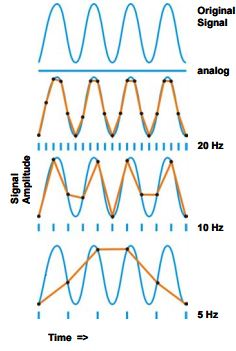
\includegraphics[scale=1.0]{figures/bProblemanalyse/samplingsfrekvens.JPEG}
	\caption{På figuren ses et eksempel på for lav samplingsfrekvens. Den øverste graf er det orginale signal, og de efterfølgende grafer, ses den orginale signale ved forskellige samplinger, hvor det kan ses at noget at signalet går tabt, ved for lav sampling. \cite{konrad2006}}
	\label{samplingsfrekvens}
\end{figure}
 
Diskretisering af amplituden betegnes som kvantisering. De enkelte samples har en amplitudeværdi og ved kvantisering inddeles denne analoge værdi i trin. I modsætning til samling sker der en approksimering i det rekonstruerede signal, da værdierne mellem to trin repræsenteres af samme digitale værdi, hvilket gør at flere værdier kan ligge indenfor den samme digitale værdi \cite{Zouridakis2003} Antallet af amplitudeniveauer, der er tilgængelige til at repræsentere det analoge signal, determineres af antal bits. F.eks. en ADC med en opløsning på 12-bit inddeles i 4096 niveauer, da $2^12$=4096. \cite{Konrad2006} Det mindste amplitudeniveau ADC'en kan opnå kaldes LSB (Least Significant Bit) og bestemmes ved følgende ligning \fxnote{kilde?? - mine noter}: 
$LSB = \frac{FSR}{(2n-1)} = \frac{FSR}/{2^n}$, hvor FSR er "full scale voltage range" \fxnote{(arbejdsområdet)}, n er antal bits, $2^n$ er antal værdier og $2^n$-1 er antal intervaller. 

Ved forstærkning er det essentielt at være opmærksom på ADC'ens \fxnote{kan man skrive det?} arbejdsområde. 
Da ADC'en har en bestemt inputområde der medfører, at et outputsignal større eller mindre end
henholdsvis den øvre og nedre værdi inden for det fastsatte område, vil blive afskåret, hvilket
vil medføre, at en del af dataen går tabt.
 \fxnote{problemer igen med at finde nogle kilder til det} 
 
%FIGUR DER ILLUSTRERER KLIPNING AF SIGNALET
%TAG UDGANGSPUNKT I NI DAQ




 